\documentclass[12pt, oneside]{article}

%Codificación e idioma
\usepackage[T1]{fontenc}
\usepackage[spanish]{babel}
\usepackage[utf8]{inputenc}

% Url
\usepackage{url}

% Graphics
\usepackage[pdftex]{graphicx}
\DeclareGraphicsExtensions{.png,.jpg}

\usepackage{wrapfig}

% Soporte multicolumna
\usepackage{multicol}

%Resaltado de sintaxis
\usepackage{color}
\definecolor{gray97}{gray}{.97}
\definecolor{gray75}{gray}{.75}
\definecolor{gray45}{gray}{.45}

\definecolor{red}{rgb}{0.6,0,0} % strings
\definecolor{green}{rgb}{0.25,0.5,0.35} % comments
\definecolor{purple}{rgb}{0.5,0,0.35} % keywords
\definecolor{blue}{rgb}{0.25,0.35,0.75} % doc

\usepackage{listings}
\lstset {
	frame				=	Ltb,
    framerule			=	0pt,
    aboveskip			=	0.5cm,
    framextopmargin		=	3pt,
    framexbottommargin	=	3pt,
    framexleftmargin	=	0.4cm,
    framesep			=	0pt,
    rulesep				=	.4pt,
    backgroundcolor		=	\color{gray97},
    rulesepcolor		=	\color{black},
    %
    stringstyle			=	\color{red},
    showstringspaces	=	false,
    basicstyle			=	\ttfamily\small,
    commentstyle		=	\color{green},
    morecomment         =   [s][\color{blue}]{/*}{*/},
    keywordstyle		=	\color{purple}\bfseries,
    tabsize					=	3,
    %
    numbers				=	left,
    numbersep			=	15pt,
    numberstyle			=	\tiny,
    numberfirstline		=	false,
    breaklines			=	true,
}

\title{Apache Torque}
\author{
	Francisco J. Serrano\\
	Benjamín Fernández\\
	Juan María Frías\\
	David Doña\\
	Enrique Ríos
}

\begin{document}

% Portada
\begin{titlepage}
	\maketitle
\end{titlepage}

% Indice generado
\tableofcontents
\newpage

\section{Introducción}
	\subsection{Fundación Apache}
		\begin{wrapfigure}{L}{0.3\textwidth}
	
\includegraphics[scale=.8]{img/apache-logo.png}
\end{wrapfigure}

Apache Software Foundation (ASF) es una organización no lucrativa (en concreto, una fundación) creada para dar soporte a los proyectos de software bajo la denominación Apache, incluyendo el popular servidor HTTP Apache. La ASF se formó a partir del llamado Grupo Apache y fue registrada en Delaware (Estados Unidos), en junio de 1999.

Apache Software Foundation es una comunidad descentralizada de desarrolladores que trabajan cada uno en sus propios proyectos de código abierto. Los proyectos Apache se caracterizan por un modelo de desarrollo basado en el consenso, la colaboración y en una licencia de software abierta y pragmática.

	\subsection{Apache Torque}
		\begin{wrapfigure}{L}{0.4\textwidth}
	
\includegraphics[scale=.8]{img/torque-logo.png}
\end{wrapfigure}

Apache Torque es un mapeador objeto relacional para Java. En otras palabras, Torque te permite acceder y manipular información en una base de datos relacional usando objetos. 
%A diferencia de la mayoría de los otros mapeadores objeto-relacional, Torque no utiliza la reflexión para tener acceso a las clases proporcionadas por el usuario, pero genera las clases necesarias (incluyendo los Objetos) a partir de un esquema XML que describe el diseño de base de datos (que puede ser escrito a mano o generado a partir de una base de datos existente)
El esquema XML puede ser usado para generar y ejecutar un script SQL el cual creará todas la tablas en la base de datos.

As Torque hides database-specific implementation details, Torque makes an application independent of a specific database if no exotic features of the database are used.
Usage of autogeneration eases the customization of the database layer, as you can override the autogenerated methods and thus easily change their behaviour.

\subsubsection{Runtime}
Torque Runtime contiene todo lo necesario para permitir a la aplicación acceder a la base de datos. Es el único componente que Torque necesita en la aplicación y puede ser usado de forma independiente.

\subsubsection{Generator}
Generator contiene las tareas de Ant las cuales hacen todo el trabajo para el plugin Maven. En el caso de usar el plugin Maven, no es necesario usar Generator directamente. No obstante, Generator puede ser llamado directamente desde Ant.

\subsubsection{Ant}

\begin{wrapfigure}{L}{0.3\textwidth}
	
\includegraphics[scale=.9]{img/ant-logo.png}
\end{wrapfigure}

Apache Ant es una libreria de Java y una herramienta de linea de comando cuya misión es
Apache Ant is a Java library and command-line tool whose mission is to drive processes described in build files as targets and extension points dependent upon each other. The main known usage of Ant is the build of Java applications. Ant supplies a number of built-in tasks allowing to compile, assemble, test and run Java applications. Ant can also be used effectively to build non Java applications, for instance C or C++ applications. More generally, Ant can be used to pilot any type of process which can be described in terms of targets and tasks. Ant is written in Java. Users of Ant can develop their own "antlibs" containing Ant tasks and types, and are offered a large number of ready-made commercial or open-source "antlibs". Ant is extremely flexible and does not impose coding conventions or directory layouts to the Java projects which adopt it as a build tool.

\subsubsection{Maven Plugin}

\begin{wrapfigure}{L}{0.3\textwidth}
	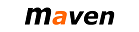
\includegraphics[scale=.8]{img/maven-logo.png}
\end{wrapfigure}

Maven plugin: Apache Maven is a software project management and comprehension tool. Based on the concept of a project object model (POM), Maven can manage a project's build, reporting and documentation from a central piece of information. (Nosotros no lo usaremos)

\subsubsection{Templates}
The templates contain the building blocks used by the generator to create the O/R peer and object classes, SQL scripts and the like. You can change the templates if you want to customize the output of the generator (this is only necessary in very special circumstances). Up to release 3.1.x, the templates were a part of the generator. Starting with the 3.2 release of Torque, the templates have been separated into their own jar archive.

\subsubsection{Village}
Village is a 100\% Pure Java API that sits on top of the JDBC API. El propósito de esta API es hacer mas fácil is to make it easier to interact with a JDBC compliant relational database.

\section{Gestores de bases de datos}

	\subsection{Postgresql}
		\begin{wrapfigure}{L}{0.3\textwidth}
	
\includegraphics[scale=.8]{img/postgresql-logo.png}
\end{wrapfigure}

PostgreSQL es un sistema de gestión de bases de datos objeto-relacional, distribuido bajo licencia BSD y con su código fuente disponible libremente. Es el sistema de gestión de bases de datos de código abierto más potente del mercado.
PostgreSQL utiliza un modelo cliente/servidor y usa multiprocesos en vez de multihilos para garantizar la estabilidad del sistema. Un fallo en uno de los procesos no afectará el resto y el sistema continuará funcionando.

	\subsection{MySQL}
		\begin{wrapfigure}{L}{0.35\textwidth}
	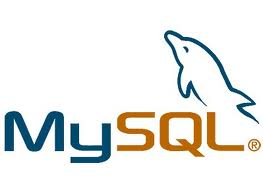
\includegraphics[scale=.3]{img/mysql-logo.jpg}
\end{wrapfigure}

MySQL es un sistema de gestión de base de datos relacional cuya licencia se ofrece bajo GNU GPL.
MySQL usa un sistema multihilo y funciona sobre una gran cantidad de plataformas.
En aplicaciones web hay baja concurrencia en la modificación de datos y en cambio el entorno es intensivo en lectura de datos, lo que hace a MySQL ideal para este tipo de aplicaciones gracias a su motor no transaccional MyISAM.
	
	\subsection{SQL Server}
		\begin{wrapfigure}{L}{0.35\textwidth}
	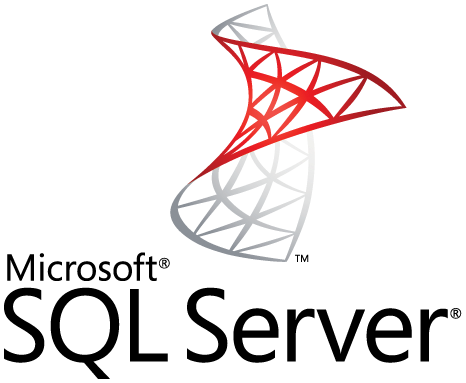
\includegraphics[scale=.25]{img/sqlserver-logo.png}
\end{wrapfigure}

Microsoft SQL Server es un sistema para la gestión de bases de datos producido por Microsoft basado en el modelo relacional. Sus lenguajes para consultas son T-SQL y ANSI SQL. Microsoft SQL Server constituye la alternativa de Microsoft a otros potentes sistemas gestores de bases de datos como son Oracle, PostgreSQL o MySQL.

\section{Instalando y configurando Apache Torque con Postgresql}
	En primer lugar descargar todo el software necesario:

\begin{description}
	\item[Runtime] \url{http://apache.rediris.es/db/torque/torque-3.3/binaries/torque-3.3.tar.gz}
	\item[Generator] \url{http://ftp.udc.es/apache/db/torque/torque-3.3/binaries/torque-gen-3.3.tar.gz}
	\item[Village] \url{http://apache.rediris.es/db/torque/torque-3.3/binaries/village-3.3.tar.gz}
	\item[Ant] \url{http://ftp.udc.es/apache//ant/binaries/apache-ant-1.8.4-bin.zip}
\end{description}

	\subsection{Instalando Ant}
		Los pasos para instalar {\bf Ant} son los siguientes:

\begin{enumerate}
	\item Descargar Ant
	\item Descomprimir el fichero obtenido en un directorio. {\em Para nuestro ejemplo hemos elegido C:}
	\item Renombrar la carpeta descomprimida {\bf apache-ant-1.8.4} como {\bf ant}, con el objetivo de hacer más sencillo el trabajo en linea de comandos.
	\item Ejecutar la consola e introducir las siguientes variables de entorno:


	\begin{itemize}
		\item Para {\bf \small ANT\_ HOME}:
		\begin{lstlisting}
		set ANT_HOME= C:\ant
		\end{lstlisting}

		\item Y para {\bf \small JAVA\_ HOME} introducir la ruta de la máquina virtual de Java. {\em En nuestro caso el comando sería el siguiente:}
		\begin{lstlisting}
		set JAVA_HOME C:\Program Files\Java\jdk1.7.0_07
		\end{lstlisting}

		\item Introducir la dirección del directorio {\bf ant} en el PATH:
		\begin{lstlisting}
		set PATH=%PATH%;%ANT_HOME%\bin
		\end{lstlisting}
	\end{itemize}
	
	\item Obtener las dependencias de bibliotecas de Ant:
	
	\begin{itemize}
		\item Desde cmd.exe nos dirigimos al directorio de Ant
		\item Ejecutar:  
		\begin{lstlisting}
		ant -f fetch.xml -Ddest=system
		\end{lstlisting}
	\end{itemize}
\end{enumerate}

Instalación de {\bf Ant} finalizada, ya podemos usar {\bf Ant} desde consola.

	\subsection{Creando un proyecto}
		\begin{enumerate}
	\item Crear un nuevo proyecto en eclipse.
	\item En el interior de la carpeta del proyecto descomprimir los siguientes paquetes:
	\begin{itemize}
		\item runtime
		\item generator
		\item village
	\end{itemize}
\end{enumerate}

	\subsection{Configurando y ejecutando Generator}
		Acceder a la carpeta {\bf torque-gen-3.3} de nuestro proyecto, una vez allí:

\begin{enumerate}
	\item Descargar el driver {\bf JDBC} de la base de datos que desee utilizar, en nuestro caso {\em Postgresql}, desde la siguiente dirección: url{http://jdbc.postgresql.org/}
	\item Introducir el driver {\bf JDBC} en el directorio {\bf lib} de Generator, que se encuentra dentro del directorio {\bf torque-gen-3.3}.

	\item Crear usuaro, password y base de datos cuyo propietario sea el usuario creado. {\em En nuestro ejemplo, en PostgreSQL, hemos usado:}
	\begin{itemize}
		\item Crear usuario y password: {\em user1} y {\em user1}, respectivamente. 
		\item Crear una base de datos, llamada {\em coches}, de la que es propietario {\em user1}.
	\end{itemize}
	
	\item Crear un directorio {\bf en la raíz del proyecto} llamado {\em schema}, donde introducir el archivo xml. En este archivo se describirá la base de datos.
	
	\item Editar el archivo {\bf build.propierties} añadiendo la configuración de nuestro proyecto.
\end{enumerate}

		\subsubsection{Editando build.propierties}
			El fichero {\bf build.propierties} es un extenso fichero en texto plano estructurado en apartados.

A continuación verá las lineas que han sido necesarias modificar para que el ejemplo {\em coches} funcione correctamente.

En el apartado {\bf PROYECT}, se ha modificado el nombre de proyecto. {\bf Apache Torque} usará {\em el nombre de proyecto} como base tanto para buscar el fichero xml así como nombre base para generar archivos del proyecto.
\begin{lstlisting}
# Nombre de nuestro proyecto
torque.project = coches
\end{lstlisting}

En el apartado {\bf TARGET DATABASE} buscaremos una línea para asignar como valor el nombre de la base de datos que deseemos utilizar. Las opciones disponibles son:

\begin{multicols}{2}
\begin{itemize}
	\item axion
	\item cloudscape
	\item db2
	\item db2400
	\item hypersonic
	\item interbase
	\item msaccess
	\item mssql
	\item mysql
	\item oracle
	\item postgresql
	\item sapdb
	\item sybase
\end{itemize}
\end{multicols}

En nuestro ejemplo usuaremos {\bf PostgreSQL}, por lo que la variable quedaría definida:
\begin{lstlisting}
# Gestor de bases de datos que vamos a usar
torque.database = postgresql
\end{lstlisting}

En el apartado {\bf DATABASE SETTINGS}, configuraremos las opciones de conexión del JDBC. Estos datos son usados por {\bf Ant} para inicializar el sistema Torque con el SQL generado.
\begin{lstlisting}
# Direcciones de acceso a la base de datos y puerto de escucha
torque.database.createUrl = jdbc:postgresql://127.0.0.1:5432/coches
torque.database.buildUrl = jdbc:postgresql://127.0.0.1:5432/coches
torque.database.url = jdbc:postgresql://127.0.0.1:5432/coches

# Driver para acceder a la base de datos
torque.database.driver = org.postgresql.Driver

# Usuario y password para acceder a la base de datos
torque.database.user = user1
torque.database.password = user1

#Direccion del host donde se encuentra la base de datos
torque.database.host = 127.0.0.1

# Direccion donde se generaran los ficheros .java y .sql
torque.output.dir = ../src

# Direccion desde donde se obtendra el esquema .xml de la base de datos
torque.schema.dir = ../schema
\end{lstlisting}

		\subsubsection{Editando coches-schema.xml}
			Ahora creamos un archivo XML llamado {\bf coches-schema.xml}, en el directorio {\bf schema}, donde describiremos la estructura de la base de datos de nuestro sistema.
{\em En este ejemplo solo se usará una tabla, más adelante se explicará las diferentes configuraciones de este fichero. La tabla usada es la siguiente:}

\begin{lstlisting}[language=xml]
<!DOCTYPE database SYSTEM "http://db.apache.org/torque/dtd/database_3_3.dtd">

<database name="coches">
	<table name="coche" description="Tabla de coches">
	<column
		name="coche_id"
		required="true"
		primaryKey="true"
		type="INTEGER"
		description="Identificador de coches"/>
	<column
		name="nombre"
		required="true"
		type="VARCHAR"
		size="128"
		description="Nombre del coche"/>
	</table>
</database>
\end{lstlisting}

Desde cmd.exe accedemos al directorio {\bf torque-gen-3.3} y ejecutamos las siguientes instrucciones:
\begin{enumerate}
	\item Esta instrucción genera los archivos .java y .sql en la carpeta que hemos indicado antes en nuestro archivo {\em build.propierties}, en nuestro caso en {\em src}:
	\begin{lstlisting}
	ant -f build-torque.xml
	\end{lstlisting}
	 
	\item La siguiente crea y configura la base de datos:
	\begin{lstlisting}
	ant -f build-torque.xml create-db
	\end{lstlisting}
	
	\item Por último esta instrucción crea las tablas en la base de datos, ejecutando el .sql creado con anterioridad: 
	\begin{lstlisting}
	ant -f build-torque.xml insert-sql
	\end{lstlisting}
\end{enumerate}

Ya tenemos en la carpeta {\em src} dos subcarpetas, una llamada {\em java} donde se encuentran los fuentes de nuestro proyecto; y otra llamada {\em sql}, donde se encuentran los scripts de generación de la base de datos. Movemos la carpeta {\em sql} a la raíz del proyecto, ya que no la necesitaremos.

Finalmente movemos el contenido del directorio {\em java} al directorio {\em src} y eliminamos el directorio {\em java}. Ya tenemos el proyecto preparado, para seguir trabajando desde Eclipse.

	\subsection{Configuración del proyecto desde Eclipse}
Como podemos observar existen numerosos errores en nuestro proyecto, ello es debido a la falta de las librerías de Torque y Village. Las añadimos desde las siguientes direcciones:

\begin{lstlisting}
coches\torque-3.3\lib
\end{lstlisting}

	\begin{center}
		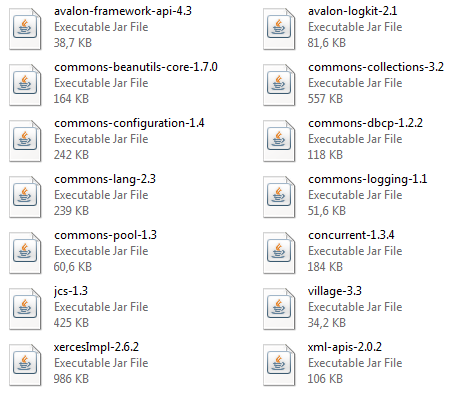
\includegraphics[height=8cm]{img/torque-lib.png}
	\end{center}
	
\begin{lstlisting}
coches\torque-3.3\
\end{lstlisting}

	\begin{center}
		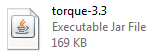
\includegraphics{img/torque-file.png}
	\end{center}
	
	Ahora ya no existen errores en el proyecto y podemos realizar una pequeña prueba de ejecución, para ello podemos crear un paquete, donde crearemos una clase Main e introduciremos el siguiente código:
	
	\begin{lstlisting}[language=java]
import java.util.Iterator;
import java.util.List;

import org.apache.torque.Torque;
import org.apache.torque.TorqueException;
import org.apache.torque.util.Criteria;

import torque.generated.Coche;
import torque.generated.CochePeer;

public class Main 
{
	public static void main(String[] args)
	{
		/*Aqui inicializamos Torque*/
		try
		{
			Torque.init("Torque.properties");
		} 
		catch (TorqueException e) 
		{	
			e.printStackTrace();
		}
		/*Aqui probamos la conexion con la base de datos*/
		try 
		{
			Coche c = new Coche();
			c.setCocheId(3);
			c.setNombre("mondeo");
			c.save();

			Coche c1 = new Coche();
			c1.setCocheId(4);
			c1.setNombre("jumpy");
			c1.save();

		} 
		catch (Exception e) 
		{
			e.printStackTrace();
		}

		/*Aqui recuperamos los datos y los mostramos por pantalla*/
		try 
		{
			Criteria crit = new Criteria();

			List<Coche> coches = CochePeer.doSelect(crit);
			for (Iterator<Coche> i = coches.iterator(); i.hasNext();)
			{
				Coche c = (Coche) i.next();
				System.out.println("coche_id: " + c.getCocheId());
				System.out.println("nombre:  " + c.getNombre()); 
				System.out.println();
			}
		} 
		catch (TorqueException e) 
		{
			e.printStackTrace();
		}
	}
}
\end{lstlisting}
	
	Desde nuestro main debemos de inicializar Torque, para ello hemos insertado la línea de código: 
	\begin{lstlisting}[language=java]
	Torque.init("Torque.properties")
	\end{lstlisting} 
	
	{\bf Toque.init} toma como parámetro un fichero llamado {\bf Torque.properties}, situado en la carpeta {\bf torque-3.3}. Movemos ese archivo a la raíz del proyecto (para que sea accesible directamente), y procedemos a configurarlo. En amarillo se encuentran las líneas que han sido modificadas con respecto al archivo de configuración por defecto.
	
	\begin{lstlisting}
# Licensed to the Apache Software Foundation (ASF) under one
# or more contributor license agreements.  See the NOTICE file
# distributed with this work for additional information
# regarding copyright ownership.  The ASF licenses this file
# to you under the Apache License, Version 2.0 (the
# "License"); you may not use this file except in compliance
# with the License.  You may obtain a copy of the License at
#
#   http://www.apache.org/licenses/LICENSE-2.0
#
# Unless required by applicable law or agreed to in writing,
# software distributed under the License is distributed on an
# "AS IS" BASIS, WITHOUT WARRANTIES OR CONDITIONS OF ANY
# KIND, either express or implied.  See the License for the
# specific language governing permissions and limitations
# under the License.

# Directorio del proyecto
torque.applicationRoot = .

# ###########
#
#  L O G G I N G
#
# ###########
# We use Log4J for all Torque logging and we embed the log4j
# properties within our application configuration.
# ###########

# This first category is required and the category
# must be named 'default'. This is used for all logging
# where an explicit category is not specified.

# Configuraciones de logging
log4j.category.org.apache.torque = ALL, org.apache.torque
log4j.appender.org.apache.torque = org.apache.log4j.FileAppender
log4j.appender.org.apache.torque.file = ${torque.applicationRoot}/logs/torque.log
log4j.appender.org.apache.torque.layout = org.apache.log4j.PatternLayout
log4j.appender.org.apache.torque.layout.conversionPattern = %d [%t] %-5p %c - %m%n
log4j.appender.org.apache.torque.append = false

# ###########
#
#  D E F A U L T S
#
# ###########
#
# These values kick in, if you don't explicitly override them in your
# various database settings. At the moment they're only used if you
# configure the SharedPoolDataSourceFactory of the PerUserDataSourceFactory
# as your data source provider. It does not work with JNDI.
#
# The example is shown for SharedPoolDataSource.
#
# ###########

# Time to wait for a connection to the database in milliseconds.
torque.defaults.pool.maxWait = 10000

# Maximum number of idle and active connections cached in a database
# definition.
# Note that, if you have multiple database definitions which access the
# same database URL, they don't share the connections but you have
# multiple pools and each has this maximum number. So if you have a
# connection licensed database engine, you must multiply this number by
# the number of times you use a specific database URL.

torque.defaults.pool.maxIdle = 8
torque.defaults.pool.maxActive = 10

# How often the pool is checked for connection which stayed in the pool
# for too long. Defaults to 5 minutes (5 * 60 * 1000)
# remove property if the idle object evictor should not be run

torque.defaults.pool.timeBetweenEvictionRunsMillis= 300000

# Lifetime of an idle connection in the pool in milliseconds.
# Defaults to one hour (1000 * 60 * 60)

torque.defaults.pool.minEvictableIdleTimeMillis = 3600000

# Sets the driver for the data sources.
# Driver de la base de datos
torque.defaults.connection.driver = org.postgresql.Driver

# Sets the URL for the datasources

# URL de la base de datos
torque.defaults.connection.url = jdbc:postgresql://127.0.0.1:5432/coches

# Sets login and password for the data sources.

# Usuario y password para acceder a la base de datos coches
torque.defaults.connection.user = user1
torque.defaults.connection.password = user1

# ###########
#
#  T O R Q U E  P R O P E R T I E S
#
# ###########
# These are your database settings. Look in the
# org.apache.torque.pool.* packages for more information.
#
# The parameters to connect to the default database.  You MUST
# configure these properly.
# ###########

# Nombre de la base de datos
torque.database.default=coches

# Gestor de base de datos
torque.database.coches.adapter=postgresql

# # Using commons-dbcp
torque.dsfactory.coches.factory=org.apache.torque.dsfactory.SharedPoolDataSourceFactory
# torque.dsfactory.coches.factory=org.apache.torque.dsfactory.PerUserPoolDataSourceFactory
torque.dsfactory.coches.pool.maxIdle=8
torque.dsfactory.coches.pool.maxActive=10
torque.dsfactory.coches.pool.testOnBorrow=true
torque.dsfactory.coches.pool.validationQuery=SELECT 1
torque.dsfactory.coches.connection.driver = org.postgresql.Driver
torque.dsfactory.coches.connection.url = jdbc:postgresql://127.0.0.1:5432/coches
torque.dsfactory.coches.connection.user = user1
torque.dsfactory.coches.connection.password = user1

# # Using jndi
# torque.dsfactory.coches.factory=org.apache.torque.dsfactory.JndiDataSourceFactory
# torque.dsfactory.coches.jndi.path=jdbc/coches
# torque.dsfactory.coches.jndi.java.naming.factory.initial = org.apache.naming.java.javaURLContextFactory
# torque.dsfactory.coches.jndi.java.naming.factory.url.pkgs = org.apache.naming

# torque.dsfactory.coches.datasource.dataSourceName=jdbc/DBcoches
# torque.dsfactory.coches.datasource.jndiEnvironment.java.naming.factory.initial = org.apache.naming.java.javaURLContextFactory
# torque.dsfactory.coches.datasource.jndiEnvironment.java.naming.factory.url.pkgs = org.apache.naming
# torque.dsfactory.coches.datasource.maxIdle=8
# torque.dsfactory.coches.datasource.maxActive=10

# # ConnectionPoolDataSource
# torque.dsfactory.coches.factory=org.apache.torque.dsfactory.JndiDataSourceFactory
# torque.dsfactory.coches.jndi.path=jdbc/DBcoches
# torque.dsfactory.coches.jndi.java.naming.factory.initial = org.apache.naming.java.javaURLContextFactory
# torque.dsfactory.coches.jndi.java.naming.factory.url.pkgs = org.apache.naming
# torque.dsfactory.coches.datasource.classname=org.apache.commons.dbcp.cpdsadapter.DriverAdapterCPDS
# torque.dsfactory.coches.datasource.driver = org.gjt.mm.mysql.Driver
# torque.dsfactory.coches.datasource.url = jdbc:mysql://localhost:3306/torque
# torque.dsfactory.coches.datasource.user = user
# torque.dsfactory.coches.datasource.password = password

# Determines if the quantity column of the IDBroker's id_table should
# be increased automatically if requests for ids reaches a high
# volume.

torque.idbroker.clever.quantity=true

# Determines whether the managers cache instances of the business objects.
# And also whether the MethodResultCache will really cache results.

torque.manager.useCache = true
\end{lstlisting}
	
	Como último paso añadimos el driver de la base de datos a nuestro proyecto en Eclipse, situado en:
	
\begin{lstlisting}
coches\torque-gen-3.3\lib
\end{lstlisting}

	\begin{center}
		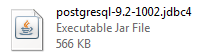
\includegraphics{img/postgresql-file.png}
	\end{center}

	Ya finalmente podemos ejecutar el proyecto, la salida por pantalla sería la siguiente: 
	
	\begin{lstlisting}
	coche_id: 3
	nombre:  mondeo

	coche_id: 4
	nombre:  jumpy
	\end{lstlisting}
	
\section{Instalando y cofigurando Apache Torque con MySQL}
La instalación bajo MySQL es muy parecida a la de Postgresql. A continuación se detallan los cambios y diferencias respecto a la instalación sobre Postgresql.

\subsection{Configuración y ejecución de Generator}
El driver JDBC de la base de datos que descargamos en esta ocasión es para MySQL, desde la siguiente dirección: \url{http://dev.mysql.com/downloads/connector/j/} y lo introducimos en la carpeta “lib” de Generator.

En la edición del archivo build.propierties, se realizan las siguientes modificaciones:
\begin{lstlisting}
# -------------------------------------------------------------------
# This is the name of your Torque project. Your non-Java generated
# files will be named using the project name selected below. If your
# project=killerapp then you will have a generated:
#
#   killerapp-schema.sql
#
# The custom is then to also rename your project XML schema from
# project-schema.xml to killerapp-schema.xml. This is required
# for a few targets such as datasql, datadump, and datadtd.
# -------------------------------------------------------------------

# Nombre de nuestro proyecto
torque.project = coches


# -------------------------------------------------------------------
#
#  T A R G E T  D A T A B A S E
#
# -------------------------------------------------------------------
# This is the target database, only considered when generating
# the SQL for your Torque project. Your possible choices are:
#
#   axion, cloudscape, db2, db2400, hypersonic, interbase, msaccess
#   mssql, mysql, oracle, postgresql, sapdb, sybase
# -------------------------------------------------------------------

# Gestor de bases de datos que vamos a usar
torque.database = mysql


# -------------------------------------------------------------------
#
#  O B J E C T  M O D E L  I N F O R M A T I O N
#
# -------------------------------------------------------------------
# These settings will allow you to customize the way your
# Peer-based object model is created.
# -------------------------------------------------------------------
# addGetByNameMethod
#   If true, Torque adds methods to get database fields by name/position.
#
# addIntakeRetrievable
#   If true, the data objects will implement Intake's Retrievable
#   interface
#
# addSaveMethod
#   If true, Torque adds tracking code to determine how to save objects.
#
# addTimeStamp
#   If true, Torque true puts time stamps in generated om files.
#
# basePrefix
#   A string to pre-pend to the file names of base data and peer objects.
#
# complexObjectModel
#   If true, Torque generates data objects with collection support and
#   methods to easily retreive foreign key relationships.
#
# targetPackage
#   Sets the Java package the om files will generated to, e.g.
#   "com.company.project.om".
#
# useClasspath
#   If true, Torque will not look in the <code>templatePath</code> directory,
#   for templates, but instead load them from the classpath, allowing you to
#   use Torque without extracted it from the jar.
#
# useManagers
#   If true, Torque will generate Manager classes that use JCS for caching.
#   Still considered experimental.
#
# objectIsCaching
#   If true, Torque generates data objects that cache their foreign
#   key relationships. If this is not desired (because the underlying objects
#   can be manipulated from other code), set this property to false. This currently
#   cannot combined with the manager setting from above.
#
# silentDbFetch
#   If true, the getXXX() methods which retrieve associated objects
#   will fetch the associated objects silently. If false, only the
#   methods where a connection is specified explicitly will
#   fetch the associated objects silently; the methods where no connection
#   is specified will not do a silent fetch and return null if no previous
#   explicit fetch was made.
#   This setting has no effect if objectIsCaching is set to false.
#
# generateBeans
#   If true, Torque will generate an additional bean for each data object,
#   plus methods to create beans from data objects and vice versa
#
# beanSuffix
#   A String to append to the class name of generated beans (if they are generated)
#
# enableJava5Features
#   If true, the generator will use Java5 generics in the generated code.
# -------------------------------------------------------------------
# Paquete donde generara el codigo
torque.targetPackage = torque.generated

# Metodos que queremos que se implementen
torque.addGetByNameMethod = true
torque.addIntakeRetrievable = false
torque.addSaveMethod = true
torque.addTimeStamp = true
torque.basePrefix = Base
torque.complexObjectModel = true
torque.useClasspath = true
torque.useManagers = false
torque.objectIsCaching = true
torque.silentDbFetch = true
torque.generateBeans = false
torque.beanSuffix = Bean
torque.enableJava5Features = false

# -------------------------------------------------------------------
#
#  D A T A B A S E  S E T T I N G S
#
# -------------------------------------------------------------------
# JDBC connection settings. This is used by the JDBCToXML task that
# will create an XML database schema from JDBC metadata. These
# settings are also used by the SQL Ant task to initialize your
# Torque system with the generated SQL.
#
# sameJavaName
#   If true, the JDBC task will set the javaName attribute for the tables
#   and columns to be the same as SQL name.
# -------------------------------------------------------------------

# Direcciones de acceso a la base de datos y puerto de escucha
torque.database.createUrl = jdbc:mysql://127.0.0.1:5432/coches
torque.database.buildUrl = jdbc:mysql://127.0.0.1:5432/coches
torque.database.url = jdbc:mysql://127.0.0.1:5432/coches
# Driver para acceder a la base de datos
torque.database.driver = org.gjt.mm.mysql.Driver
# Usuario y password para acceder a la base de datos
torque.database.user = user1
torque.database.password = user1
#Direccion del host donde se encuentra la base de datos
torque.database.host = 127.0.0.1

torque.sameJavaName = false

# Direccion donde segeneraran los ficheros .java y .sql
torque.output.dir = ../src
# Direccion desde donde se obtendra el esquema .xml de la base de datos
torque.schema.dir = ../schema
\end{lstlisting}

\subsection{Configuración del proyecto desde eclipse}
Las propiedades del archivo Torque.properties son como siguen para MySQL:

\begin{lstlisting}
# Directorio del proyecto
torque.applicationRoot = .

# ###########
#
#  L O G G I N G
#
# ###########
# We use Log4J for all Torque logging and we embed the log4j
# properties within our application configuration.
# ###########

# This first category is required and the category
# must be named 'default'. This is used for all logging
# where an explicit category is not specified.

# Configuraciones de logging
log4j.category.org.apache.torque = ALL, org.apache.torque
log4j.appender.org.apache.torque = org.apache.log4j.FileAppender
log4j.appender.org.apache.torque.file = ${torque.applicationRoot}/logs/torque.log
log4j.appender.org.apache.torque.layout = org.apache.log4j.PatternLayout
log4j.appender.org.apache.torque.layout.conversionPattern = %d [%t] %-5p %c - %m%n
log4j.appender.org.apache.torque.append = false

# ###########
#
#  D E F A U L T S
#
# ###########
#
# These values kick in, if you don't explicitly override them in your
# various database settings. At the moment they're only used if you
# configure the SharedPoolDataSourceFactory of the PerUserDataSourceFactory
# as your data source provider. It does not work with JNDI.
#
# The example is shown for SharedPoolDataSource.
#
# ###########

# Time to wait for a connection to the database in milliseconds.
torque.defaults.pool.maxWait = 10000

# Maximum number of idle and active connections cached in a database
# definition.
# Note that, if you have multiple database definitions which access the
# same database URL, they don't share the connections but you have
# multiple pools and each has this maximum number. So if you have a
# connection licensed database engine, you must multiply this number by
# the number of times you use a specific database URL.

torque.defaults.pool.maxIdle = 8
torque.defaults.pool.maxActive = 10

# How often the pool is checked for connection which stayed in the pool
# for too long. Defaults to 5 minutes (5 * 60 * 1000)
# remove property if the idle object evictor should not be run
torque.defaults.pool.timeBetweenEvictionRunsMillis= 300000

# Lifetime of an idle connection in the pool in milliseconds.
# Defaults to one hour (1000 * 60 * 60)

torque.defaults.pool.minEvictableIdleTimeMillis = 3600000

# Sets the driver for the data sources.

# Driver de la base de datos
torque.defaults.connection.driver = org.gjt.mm.mysql.Driver

# Sets the URL for the datasources

# URL de la base de datos
torque.defaults.connection.url = jdbc:mysql://127.0.0.1:5432/coches

# Sets login and password for the data sources.

# Usuario y password para acceder a la base de datos coches
torque.defaults.connection.user = user1
torque.defaults.connection.password = user1

# ###########
#
#  T O R Q U E  P R O P E R T I E S
#
# ###########
# These are your database settings. Look in the
# org.apache.torque.pool.* packages for more information.
#
# The parameters to connect to the default database.  You MUST
# configure these properly.
# ###########

# Nombre de la base de datos
torque.database.default=coches

# Gestor de base de datos
torque.database.coches.adapter=mysql

# # Using commons-dbcp
torque.dsfactory.coches.factory=org.apache.torque.dsfactory.SharedPoolDataSourceFactory
# torque.dsfactory.coches.factory=org.apache.torque.dsfactory.PerUserPoolDataSourceFactory
torque.dsfactory.coches.pool.maxIdle=8
torque.dsfactory.coches.pool.maxActive=10
torque.dsfactory.coches.pool.testOnBorrow=true
torque.dsfactory.coches.pool.validationQuery=SELECT 1
torque.dsfactory.coches.connection.driver = org.gjt.mm.mysql.Driver
torque.dsfactory.coches.connection.url = jdbc:mysql://127.0.0.1:5432/coches
torque.dsfactory.coches.connection.user = user1
torque.dsfactory.coches.connection.password = user1

# # Using jndi
# torque.dsfactory.coches.factory=org.apache.torque.dsfactory.JndiDataSourceFactory
# torque.dsfactory.coches.jndi.path=jdbc/coches
# torque.dsfactory.coches.jndi.java.naming.factory.initial = org.apache.naming.java.javaURLContextFactory
# torque.dsfactory.coches.jndi.java.naming.factory.url.pkgs = org.apache.naming

# torque.dsfactory.coches.datasource.dataSourceName=jdbc/DBcoches
# torque.dsfactory.coches.datasource.jndiEnvironment.java.naming.factory.initial = org.apache.naming.java.javaURLContextFactory
# torque.dsfactory.coches.datasource.jndiEnvironment.java.naming.factory.url.pkgs = org.apache.naming
# torque.dsfactory.coches.datasource.maxIdle=8
# torque.dsfactory.coches.datasource.maxActive=10

# # ConnectionPoolDataSource
# torque.dsfactory.coches.factory=org.apache.torque.dsfactory.JndiDataSourceFactory
# torque.dsfactory.coches.jndi.path=jdbc/DBcoches
# torque.dsfactory.coches.jndi.java.naming.factory.initial = org.apache.naming.java.javaURLContextFactory
# torque.dsfactory.coches.jndi.java.naming.factory.url.pkgs = org.apache.naming
# torque.dsfactory.coches.datasource.classname=org.apache.commons.dbcp.cpdsadapter.DriverAdapterCPDS
# torque.dsfactory.coches.datasource.driver = org.gjt.mm.mysql.Driver
# torque.dsfactory.coches.datasource.url = jdbc:mysql://localhost:3306/torque
# torque.dsfactory.coches.datasource.user = user
# torque.dsfactory.coches.datasource.password = password

# Determines if the quantity column of the IDBroker's id_table should
# be increased automatically if requests for ids reaches a high
# volume.

torque.idbroker.clever.quantity=true

# Determines whether the managers cache instances of the business objects.
# And also whether the MethodResultCache will really cache results.

torque.manager.useCache = true
\end{lstlisting}

En este caso, en driver que hay que añadir a nuestro proyecto eclipse es el siguiente:
\begin{lstlisting}
coches\orque-gen-3.3\lib
\end{lstlisting}

\begin{center}
	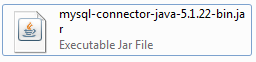
\includegraphics{img/mysql-file.png}
\end{center}

\section{Instalando y cofigurando Apache Torque con Microsoft SQL Server}
Para la instalación con MS SQL Server habrá que crear un nuevo usuario, o dar permisos a uno ya existente para el acceso a la base de datos que estemos utilizando. Este usuario debe tener la autenticación de SQL Server y el rol db\_ owner. Hay varios drivers disponibles para este tipo de base de datos, como jTDS y uno propio de MS SQL Server disponible desde su página de descargas. En esta guía explicaremos como utilizar jTDS.

\subsection{Configuración y ejecución de Generator}
En la edición del archivo build.propierties, se realizan las siguientes modificaciones:

\begin{lstlisting}
# ###########
# This is the name of your Torque project. Your non-Java generated
# files will be named using the project name selected below. If your
# project=killerapp then you will have a generated:
#
#   killerapp-schema.sql
#
# The custom is then to also rename your project XML schema from
# project-schema.xml to killerapp-schema.xml. This is required
# for a few targets such as datasql, datadump, and datadtd.
# ###########
# Nombre de nuestro proyecto
torque.project = coches


# ###########
#
#  T A R G E T  D A T A B A S E
#
# ###########
# This is the target database, only considered when generating
# the SQL for your Torque project. Your possible choices are:
#
#   axion, cloudscape, db2, db2400, hypersonic, interbase, msaccess
#   mssql, mysql, oracle, postgresql, sapdb, sybase
# ###########

# Gestor de bases de datos que vamos a usar
torque.database = mssql
torque.database.type = mssql


# ###########
#
#  O B J E C T  M O D E L  I N F O R M A T I O N
#
# ###########
# These settings will allow you to customize the way your
# Peer-based object model is created.
# ###########
# addGetByNameMethod
#   If true, Torque adds methods to get database fields by name/position.
#
# addIntakeRetrievable
#   If true, the data objects will implement Intake's Retrievable
#   interface
#
# addSaveMethod
#   If true, Torque adds tracking code to determine how to save objects.
#
# addTimeStamp
#   If true, Torque true puts time stamps in generated om files.
#
# basePrefix
#   A string to pre-pend to the file names of base data and peer objects.
#
# complexObjectModel
#   If true, Torque generates data objects with collection support and
#   methods to easily retreive foreign key relationships.
#
# targetPackage
#   Sets the Java package the om files will generated to, e.g.
#   "com.company.project.om".
#
# useClasspath
#   If true, Torque will not look in the <code>templatePath</code> directory,
#   for templates, but instead load them from the classpath, allowing you to
#   use Torque without extracted it from the jar.
#
# useManagers
#   If true, Torque will generate Manager classes that use JCS for caching.
#   Still considered experimental.
#
# objectIsCaching
#   If true, Torque generates data objects that cache their foreign
#   key relationships. If this is not desired (because the underlying objects
#   can be manipulated from other code), set this property to false. This currently
#   cannot combined with the manager setting from above.
#
# silentDbFetch
#   If true, the getXXX() methods which retrieve associated objects
#   will fetch the associated objects silently. If false, only the
#   methods where a connection is specified explicitly will
#   fetch the associated objects silently; the methods where no connection
#   is specified will not do a silent fetch and return null if no previous
#   explicit fetch was made.
#   This setting has no effect if objectIsCaching is set to false.
#
# generateBeans
#   If true, Torque will generate an additional bean for each data object,
#   plus methods to create beans from data objects and vice versa
#
# beanSuffix
#   A String to append to the class name of generated beans (if they are generated)
#
# enableJava5Features
#   If true, the generator will use Java5 generics in the generated code.
# ###########
# Paquete donde generara el codigo
torque.targetPackage = torque.generated

# Metodos que queremos que se implementen
torque.addGetByNameMethod = true
torque.addIntakeRetrievable = false
torque.addSaveMethod = true
torque.addTimeStamp = true
torque.basePrefix = Base
torque.complexObjectModel = true
torque.useClasspath = true
torque.useManagers = false
torque.objectIsCaching = true
torque.silentDbFetch = true
torque.generateBeans = false
torque.beanSuffix = Bean
torque.enableJava5Features = false

# ###########
#
#  D A T A B A S E  S E T T I N G S
#
# ###########
# JDBC connection settings. This is used by the JDBCToXML task that
# will create an XML database schema from JDBC metadata. These
# settings are also used by the SQL Ant task to initialize your
# Torque system with the generated SQL.
#
# sameJavaName
#   If true, the JDBC task will set the javaName attribute for the tables
#   and columns to be the same as SQL name.
# ###########

# Direcciones de acceso a la base de datos y puerto de escucha
torque.database.createUrl=jdbc:jtds:sqlserver://127.0.0.1:1433/template1/coches
torque.database.buildUrl = jdbc:jtds:sqlserver://:1433/coches
torque.database.url = jdbc:jtds:sqlserver://127.0.0.1:1433/coches
# Driver para acceder a la base de datos
torque.database.driver = net.sourceforge.jtds.jdbc.Driver
# Usuario y password para acceder a la base de datos
torque.database.user = user1
torque.database.password = user1
#Direccion del host donde se encuentra la base de datos
torque.database.host = 127.0.0.1

torque.sameJavaName = false

# Direccion donde segeneraran los ficheros .java y .sql
torque.output.dir = ../src
# Direccion desde donde se obtendra el esquema .xml de la base de datos
torque.schema.dir = ../schema
\end{lstlisting}

\subsection{Configuración del proyecto desde eclipse}
Las propiedades del archivo Torque.properties son de la siguiente forma en MS SQL Server:
\begin{lstlisting}
# Directorio del proyecto
torque.applicationRoot = .

# ###########
#
#  L O G G I N G
#
# ###########
# We use Log4J for all Torque logging and we embed the log4j
# properties within our application configuration.
# ###########

# This first category is required and the category
# must be named 'default'. This is used for all logging
# where an explicit category is not specified.

# Configuraciones de logging
log4j.category.org.apache.torque = ALL, org.apache.torque
log4j.appender.org.apache.torque = org.apache.log4j.FileAppender
log4j.appender.org.apache.torque.file = ${torque.applicationRoot}/logs/torque.log
log4j.appender.org.apache.torque.layout = org.apache.log4j.PatternLayout
log4j.appender.org.apache.torque.layout.conversionPattern = %d [%t] %-5p %c - %m%n
log4j.appender.org.apache.torque.append = false

# ###########
#
#  D E F A U L T S
#
# ###########
#
# These values kick in, if you don't explicitly override them in your
# various database settings. At the moment they're only used if you
# configure the SharedPoolDataSourceFactory of the PerUserDataSourceFactory
# as your data source provider. It does not work with JNDI.
#
# The example is shown for SharedPoolDataSource.
#
# ###########

# Time to wait for a connection to the database in milliseconds.
torque.defaults.pool.maxWait = 10000

# Maximum number of idle and active connections cached in a database
# definition.
# Note that, if you have multiple database definitions which access the
# same database URL, they don't share the connections but you have
# multiple pools and each has this maximum number. So if you have a
# connection licensed database engine, you must multiply this number by
# the number of times you use a specific database URL.

torque.defaults.pool.maxIdle = 8
torque.defaults.pool.maxActive = 10

# How often the pool is checked for connection which stayed in the pool
# for too long. Defaults to 5 minutes (5 * 60 * 1000)
# remove property if the idle object evictor should not be run

torque.defaults.pool.timeBetweenEvictionRunsMillis= 300000

# Lifetime of an idle connection in the pool in milliseconds.
# Defaults to one hour (1000 * 60 * 60)

torque.defaults.pool.minEvictableIdleTimeMillis = 3600000
# Sets the driver for the data sources.

# Driver de la base de datos
torque.defaults.connection.driver = net.sourceforge.jtds.jdbc.Driver

# Sets the URL for the datasources

# URL de la base de datos
torque.defaults.connection.url = jdbc:jtds:sqlserver://127.0.0.1:1433/coches

# Sets login and password for the data sources.

# Usuario y password para acceder a la base de datos coches
torque.defaults.connection.user = user1
torque.defaults.connection.password = user1

# ###########
#
#  T O R Q U E  P R O P E R T I E S
#
# ###########
# These are your database settings. Look in the
# org.apache.torque.pool.* packages for more information.
#
# The parameters to connect to the default database.  You MUST
# configure these properly.
# ###########

# Nombre de la base de datos
torque.database.default=coches

# Gestor de base de datos
torque.database.wacs.adapter=mssql

# # Using commons-dbcp
torque.dsfactory.coches.factory=org.apache.torque.dsfactory.SharedPoolDataSourceFactory
# torque.dsfactory.coches.factory=org.apache.torque.dsfactory.PerUserPoolDataSourceFactory
torque.dsfactory.coches.pool.maxIdle=8
torque.dsfactory.coches.pool.maxActive=10
torque.dsfactory.coches.pool.testOnBorrow=true
torque.dsfactory.coches.pool.validationQuery=SELECT 1
torque.dsfactory.coches.connection.driver = net.sourceforge.jtds.jdbc.Driver
torque.dsfactory.coches.connection.url = jdbc:jtds:sqlserver://127.0.0.1:1433/coches
torque.dsfactory.coches.connection.user = user1
torque.dsfactory.coches.connection.password = user1
# # Using jndi
# torque.dsfactory.coches.factory=org.apache.torque.dsfactory.JndiDataSourceFactory
# torque.dsfactory.coches.jndi.path=jdbc/coches
# torque.dsfactory.coches.jndi.java.naming.factory.initial = org.apache.naming.java.javaURLContextFactory
# torque.dsfactory.coches.jndi.java.naming.factory.url.pkgs = org.apache.naming

# torque.dsfactory.coches.datasource.dataSourceName=jdbc/DBcoches
# torque.dsfactory.coches.datasource.jndiEnvironment.java.naming.factory.initial = org.apache.naming.java.javaURLContextFactory

# Determines if the quantity column of the IDBroker's id_table should
# be increased automatically if requests for ids reaches a high
# volume.

torque.idbroker.clever.quantity=true

# Determines whether the managers cache instances of the business objects.
# And also whether the MethodResultCache will really cache results.

torque.manager.useCache = true
\end{lstlisting}

Por último se añade el driver de la base de datos a nuestro proyecto en Eclipse, situado en:
\begin{lstlisting}
coches\torque-gen-3.3\lib
\end{lstlisting}

%Falta imagen del conector java

Notas acerca el archivo de esquema XML:

Hay que tener cuidado con el uso de palabras clave de MS SQL en tablas y columnas. 
MS SQL admite poner el atributo {\em defaultIdMethod = “native”} para generar los campos automáticamente.

\section{Configuración del archivo schema.xml}
\begin{center}
	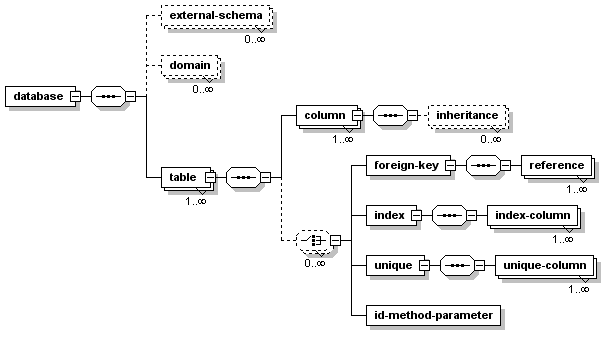
\includegraphics[height=8cm]{img/xml-config.png}
\end{center}
	
	El esquema de base de datos de torque describe los elementos y atributos de la propia base de datos que estemos utillizando. A continuación se describe los principales elementos y las bases de datos compatibles actualmente.

\subsection{Elemento Database}
Puede contener los siguientes 8 atributos:

\begin{description}
	\item[name] el nombre de la base de datos.
	\item[defaultIdMethod] este se aplica a aquellas tablas que no tienen un atributo id definido. Por defecto es “none”. Normalmente se utiliza si no quieres ID’s generados.
	\item[defaultJavaType] tipo predeterminado de las columnas de la base de datos ( “object” o “primitive”, por defecto es primitive).
	\item[package] paquete base donde se generará los modelos de objetos asociados con la base de datos. Este reemplaza la propiedad “targetPackage” del archivo build.properties de Torque.
	\item[baseClass] la clase base que se utilizará al generar el modelo de objetos.
	\item[basePeer] la clase peer a utilizar al generar los pares del modelo de objetos.
	defaultJavaNamingMethod: este atributo determina como se convierten los nombres de las tablas y columnas en una clase Java o el nombre del método. Puede tener 3 valores diferentes:
	\item[nochange] no se realizan cambios.
	\item[underscore] se elimina el subrayado, la primera letra y después de un guión se pone la letra en mayúscula, el resto de caracteres en minúscula.
	\item[javaname] con guiones bajos, pero las letras no se convierten en minúscula.
	\item[heavyIndexing] agrega indices adicionales para columnas con varias claves primarias.
\end{description}

\subsubsection{External-schema}
Incluye otro archivo de esquema. Puede haber 0 o más elementos de este tipo.

\begin{lstlisting}[language=XML]
<Externa del esquema
	filename = "extext-schema.xml" />
\end{lstlisting}

\subsubsection{Domain}
Se utiliza para definir los atributos de las columnas.Puede haber 0 o más elementos de este tipo. 

\begin{lstlisting}[language=XML]
<domain
	name="amount"
	type="NUMERIC"
	size="10"
	scale="2"
	default="0"
	description="amount domain" />
\end{lstlisting}

\subsubsection{Table}
Elemento: table
Define las tablas y sus atributos:

\begin{lstlisting}[language=XML]
<table
	name="MY_TABLE"
	javaName="table"
	idMethod="idbroker"
	skipSql="false"
	baseClass="com.myapp.om.table.BaseClass"
	basePeer="com.myapp.om.table.BasePeer"
	javaNamingMethod="underscore"
	description="Table for Torque tests">

	<!-- column information here -->

</table>
\end{lstlisting}

El elemento table tiene los siguientes atributos asociados.

name: el nombre de la tabla que está siendo referenciada.
javaName: como se llamará esta tabla en Java.
idMethod: como s e crearán las claves primarias. Por defecto es nulo.
skipSql: valor booleano (true o false) que indica si hacer o no la generación de SQL para esta referencia.
abstract: valor booleano para generar la clase como abstracta o no.
baseClass: usado para la generación de OM Peer
basePeer: usado para la generación de OM Peer.
alias: define un alias para la tabla.
interface: especifica una interfaz que debería ser referenciada en la sección “implements” de la clase generada.
javaNamingMethod: especifica el nombre de la clase Java del correspondiente objeto OM. Este atributo reemplaza al atributo “defaultJavaNamingMehtod” del elemento de la base de datos (database).
description: se utiliza para la generación de documentación.

El elemento “table” también puede contener los siguientes elementos:

\paragraph{Column}
Puede haber 1 o más elementos de este tipo por tabla.

\begin{lstlisting}[language=xml]
<column
           		name="MY_COLUMN"
           		javaName="Column"
           		primaryKey="true"
           		required="true"
           		size="4"
           		type="VARCHAR"
           		javaNamingMethod="underscore">

           		<!-- inheritance info if necessary -->
</column>
\end{lstlisting}

Contiene los siguientes atributos:
name: nombre de la columna que está siendo referenciada.
javaName: como se llamará esta columna en Java.
primaryKey: valor booleano que indica si es la clave primaria o no. (true o false)
required: indica si el valor es requerido.(true o false, por defecto es false)
type: de que tipo es la columna.
javaType: el tipo de la columna en Java.
size: cuantos carácteres o digitos van a ser almacenados.
default: valor por defecto si al insertar está vacio.
autoIncrement: si este campo tiene autoincremento no. (true o false, por defecto es false)
inheritance. Indica si tiene herencia. Puede tomar los valores “single” o “false”.

javaNamingMethod: especifica el nombre que será utilizado en la clase Java del correspondiente objeto OM. Este atributo reemplaza al atributo “defaultJavaNamingMehtod” del elemento de la base de datos (database).

description: se utiliza para la generación de documentación.

\paragraph{Foreing-key}
Puede haber 0 o más elementos de este tipo por tabla.

\begin{lstlisting}[language=xml]
<foreign-key foreignTable="MY_TABLE"
	name="MY_TABLE_FK"
	onUpdate="none"
	onDelete="none">
	
	<!-- reference info -->
	<reference
	local="[columna_local]"
	foreign="[columna_foreign]"/>
</foreign-key>
\end{lstlisting}

Este elemento tiene 4 atributos:
foreignTable: el nombre de la tabla donde se encuentra la clave foránea.
name: el nombre de la clave foránea.
onUpdate: acción a realizar cuando se actualiza el valor en foreignTable.
onDelete: acción a realizar cuando se elimina el valor en foreingTable.

\paragraph{Index}
Puede haber 0 o más elementos de este tipo por tabla.

\begin{lstlisting}[language=xml]
<index name="MY_INDEX">
	<!-- index-column info -->
</index>
\end{lstlisting}

El elemento index tiene 1 atributo asociado:
name: el nombre del índice. 
Puede contener 1 o más elementos  del tipo:

\subparagraph{Index-column}
Tiene solo un atributo: “name” que indica el nombre del índice de la columna. Este elemento no puede contener otros elementos.
\begin{lstlisting}[language=xml]
<index-column name="INDEX_COLUMN"/>
\end{lstlisting}

\section{Funcionamiento de las clases generadas}
\subsection{Usando el objeto}
Torque genera cuatro clases por cada tabla. Por ejemplo en la aplicación coche nos aparecen las siguientes clases:

\begin{description}
	\item[BaseCoche.java] Es donde Torque genera toda la lógica necesaria para la clase coche.

	\item[Coche.java] Esta clase extiende de BaseCoche.java, Torque nos proporciona esta clase vacía, para que en el caso de que necesitemos añadir nuevos métodos a Coche, lo hagamos en ella.

	\item[BaseCochePeer.java] En esta clase Torque nos proporciona métodos estáticos para el uso de la base de datos.

	\item[CochePeer.java] Al igual que en Coche.java esta clase extiende de BaseCochePeer.java y Torque nos la genera vacía para que añadamos nuestros propios métodos estáticos.
\end{description}

\subsection{Insertando filas}

Para añadir una nueva fila en la tabla “Publisher”, existen dos formas de hacerlo. Una es utilizando la clase estática generada “xPeer” (siendo ‘x’ el nombre de la tabla), y otra mediante objetos con el nombre propio de la tabla.

Para insertar una nueva fila mediante objetos, en primer lugar debemos de crear un objeto de la tabla que vamos a modificar/insertar datos.

\begin{lstlisting}[language=Java]
Publisher addison = new Publisher();
\end{lstlisting}

A continuación rellenamos los atributos del objeto, que son los mismos que las columnas de la tabla.

\begin{lstlisting}[language=Java]
addison.setName("Addison Wesley Professional");
\end{lstlisting}

Finalmente, para guardar los datos del objeto en la base de datos, llamamos al método “save()”.

\begin{lstlisting}[language=Java]
addison.save();
\end{lstlisting}

\subsection{Usando la clase estática}
Creamos un objeto de la tabla.

\begin{lstlisting}[language=Java]
Author stevens = new Author();
\end{lstlisting}

Se rellenan los campos.

\begin{lstlisting}[language=Java]
stevens.setFirstName("W.");
stevens.setLastName("Stevens");
\end{lstlisting}

Usamos la clase estática en este caso llamada “AuthorPeer”, para insertar el nuevo registro en la base de datos

\begin{lstlisting}[language=Java]
AuthorPeer.doInsert(stevens);
\end{lstlisting}


\subsection{Seleccionando filas}
La clase generada “Criteria” es la equivalente al ‘where’ de sql. Para una consulta tendremos que generar siempre un objeto Criteria, en caso de que la consulta no incluya un tipo ‘where’, simplemente se crea el objeto Criteria y no se modifica ningún atributo.

\begin{lstlisting}[language=Java]
Criteria crit = new Criteria();
\end{lstlisting}

La clase estática “xPeer” contiene métodos para la manipulación de la base de datos, como por ejemplo usaremos una consulta de selección

\begin{lstlisting}[language=Java]
List books = BookPeer.doSelect(crit);
\end{lstlisting}

Si queremos añadir alguna condición where, simplemente utilizamos el método “add”. Dicho método tiene gran variedad de cabeceras para los distintos tipos de condiciones (group by, like....). En este caso, ponemos como condición la igualdad:

\begin{lstlisting}[language=Java]
Criteria crit = new Criteria();
crit.add(BookPeer.ISBN, "0-618-12902-2");
List books = BookPeer.doSelect(crit);
\end{lstlisting}

Otro ejemplo, para una comparación “mayor que”:

\begin{lstlisting}
crit.add(CochePeer.COCHE_ID, 2, Criteria.GREATER_THAN);
\end{lstlisting}

\subsection{Actualizando filas} 

Para la actualización de filas, se puede utilizar el método ‘doUpdate’ de la clase estática ‘xPeer’:

\begin{lstlisting}[language=Java]
effective.setAuthor(stevens);
effective.save();
tcpip.setAuthor(bloch);
BookPeer.doUpdate(tcpip);
\end{lstlisting}

\subsection{Eliminando filas}

Para eliminar filas, se utiliza el método ‘doDelete’ de ‘xPeer’

\begin{lstlisting}[language=Java]
crit = new Criteria();
crit.add(BookPeer.ISBN, "0-618-12902-2");
BookPeer.doDelete(crit);

crit = new Criteria();
crit.add(BookPeer.ISBN, "0-201-63346-9");
crit.add(BookPeer.TITLE, "TCP/IP Illustrated, Volume 1");
BookPeer.doDelete(crit);
\end{lstlisting}

%Estudiar datadump
En el ant, en la última sentencia, se añade “datadump” 
‘ant -f build-torque.xml datadump’

\section{Aplicacion}
\subsection{Esquema base datos}
\begin{lstlisting}[language=xml]
<!DOCTYPE database SYSTEM
 "http://db.apache.org/torque/dtd/database_3_3.dtd">

<database name="notas">
  <table name="usuario" description="Tabla de usuarios">
    <column
      name="usuario_id"
      required="true"
      primaryKey="true"
      type="INTEGER"
      description="Identificador de usuario"/>
    <column
      name="nick"
      required="true"
      type="VARCHAR"
      size="128"
      description="nick del usuario"/>
  </table>
  <table name="nota" description="Tabla de notas">
    <column
      name="nota_id"
      required="true"
      primaryKey="true"
      type="INTEGER"
      description="Identificador de nota"/>
    <column
      name="texto"
      required="true"
      type="VARCHAR"
      size="150"
      description="texto de la nota"/>
	<column
      name="usuario_id"
      required="true"
      type="INTEGER"
      description="Clave foranea de usuario"/>
	<foreign-key foreignTable="usuario">
      <reference
        local="usuario_id"
        foreign="usuario_id"/>
    </foreign-key>
  </table>
</database>
\end{lstlisting}

\end{document}
